\documentclass[11pt,a4paper]{article}
\usepackage[utf8]{inputenc}
\usepackage[T1]{fontenc}
\usepackage[ngerman]{babel}
\usepackage{lmodern}
\usepackage{microtype}
\usepackage[margin=2.2cm]{geometry}
\usepackage{amsmath,amssymb}
\usepackage{graphicx}
\usepackage{booktabs}
\usepackage{enumitem}
\usepackage{caption}
\usepackage{xcolor}
\usepackage{tikz}
\usetikzlibrary{positioning,arrows.meta,fit}
\usepackage[most]{tcolorbox}
\usepackage[hidelinks]{hyperref}

\graphicspath{{../bilder/}}
\setlength{\parindent}{0pt}
\setlength{\parskip}{0.55em}
\setlist{itemsep=0.2em,topsep=0.3em}

\definecolor{merkfarbe}{HTML}{2a78d6}
\definecolor{achtungfarbe}{HTML}{eb6834}
\newtcolorbox{merke}{colback=merkfarbe!6,colframe=merkfarbe,boxrule=0.6pt,arc=2pt,
  left=6pt,right=6pt,top=4pt,bottom=4pt,fonttitle=\bfseries,title=Merke}
\newtcolorbox{achtung}{colback=achtungfarbe!6,colframe=achtungfarbe,boxrule=0.6pt,arc=2pt,
  left=6pt,right=6pt,top=4pt,bottom=4pt,fonttitle=\bfseries,title=Achtung}
\newcommand{\code}[1]{\texttt{#1}}

\title{\textbf{Lernskript: Nutzt unsere Spurerkennung\\ benachbarte Fahrbahnmarkierungen?}\\[4pt]
\large Alles Wichtige zum XAI-Projekt -- zum Lesen unterwegs}
\author{Brisild Capani\\\small DHBW Stuttgart · DHBW Smart Rollerz · Modul Explainable AI}
\date{Stand: \today}

\begin{document}
\maketitle

\begin{center}
\begin{minipage}{0.86\textwidth}
\small
\textbf{Wie du das Skript liest.} Die Kapitel bauen aufeinander auf: erst was das Modell tut
(1--3), dann wie wir es untersuchen (4--6), dann was herauskam und wo die Grenzen liegen
(7--8). Blaue Kästen fassen zusammen, orange Kästen warnen vor Denkfehlern. Am Ende stehen ein
Glossar und Fragen, mit denen du prüfen kannst, ob du alles verstanden hast.
\end{minipage}
\end{center}

\tableofcontents
\newpage

% =====================================================================
\section{Worum geht es überhaupt?}

Unser Modellauto fährt autonom und muss dafür die Fahrbahnmarkierungen erkennen: die linke
Linie, die gestrichelte Mittellinie und die rechte Linie. Das übernimmt ein neuronales Netz,
eine Variante von \emph{Ultra Fast Lane Detection v2} (UFLDv2).

Im echten Betrieb ist nicht immer jede Linie gut sichtbar: Sonnenlicht blendet, Schatten fallen,
ein Hindernis steht auf der Linie, Markierungen sind abgenutzt. Trotzdem findet das Modell oft
noch eine Linie. Die Frage ist: \textbf{woher weiß es, wo sie liegt?} Zwei Möglichkeiten:

\begin{enumerate}
  \item Es nutzt die \textbf{sichtbaren Reste derselben Linie}, also die Stücke oberhalb und
        unterhalb der Lücke, und verbindet sie.
  \item Es nutzt die \textbf{Nachbarlinien}: Liegt die Mittellinie hier, muss die rechte Linie
        ungefähr eine Spurbreite daneben liegen.
\end{enumerate}

Das ist die \textbf{Forschungsfrage}: \emph{Nutzt das Modell benachbarte Markierungen, um eine
teilweise verdeckte Linie zu erkennen?}

Beantwortet wird sie mit zwei Werkzeugen aus der Explainable AI (XAI):

\begin{itemize}
  \item \textbf{Verdeckungsexperimente:} Wir verändern das Bild gezielt und messen, wie sich die
        Vorhersage ändert. Das ist ein \emph{kausaler} Test: Wir greifen ein und schauen, was
        passiert.
  \item \textbf{Grad-CAM und HiResCAM:} Diese Verfahren erzeugen Heatmaps, die zeigen sollen,
        welche Bildbereiche für eine Vorhersage wichtig waren. Sie greifen nicht ein, sondern
        werten nur die Gradienten des Netzes aus.
\end{itemize}

Der eigentliche XAI-Kern des Projekts ist der Vergleich: \textbf{Zeigen die Heatmaps dasselbe
wie die Experimente?} Wenn ja, kann man den Heatmaps trauen. Wenn nein, wissen wir, dass sie
für dieses Modell irreführend sein können.

\begin{merke}
Experimente beantworten \emph{„Was passiert, wenn X fehlt?“}. Heatmaps beantworten \emph{„Wohin
zeigen die Gradienten?“}. Das ist nicht dasselbe. Unser Projekt prüft, wie gut das Zweite das
Erste vorhersagt.
\end{merke}

% =====================================================================
\section{Was das Modell sieht und was es ausgibt}

\subsection{Die Eingabe}

Die Kamera liefert ein Bild, das in eine Draufsicht umgerechnet wird (\emph{Bird's Eye View},
BEV). Die Linien laufen darin ungefähr senkrecht von unten nach oben. Die schwarzen Dreiecke an den
Rändern sind Bereiche ohne Bildinhalt, die bei der Umrechnung entstehen. Unten in der Mitte sieht
man das eigene Fahrzeug.

Das Bild ist in Graustufen. Für das Netz wird es auf drei gleiche Kanäle kopiert, auf die
Eingabegröße verkleinert und wie bei ImageNet normalisiert (Mittelwert abziehen, durch die
Standardabweichung teilen).

\subsection{Zeilenanker: die zentrale Idee von UFLD}

Klassische Spurerkennung entscheidet für jeden einzelnen Pixel, ob er zu einer Linie gehört
(\emph{Segmentierung}). Das ist rechenaufwendig. UFLD macht es anders und deshalb schneller:

\begin{itemize}
  \item Über das Bild werden \textbf{feste waagerechte Zeilen} gelegt, die \textbf{Zeilenanker}
        (beim alten Modell 35, beim 2026er 55).
  \item Jede Zeile wird in \textbf{Kästchen} (\emph{Bins}) geteilt (50 bzw. 100).
  \item Für jede Zeile und jede der drei Linien gibt das Netz jedem Kästchen eine
        \textbf{Punktzahl} (Logit). Wo die Punktzahl am höchsten ist, liegt die Linie.
  \item Zusätzlich gibt es pro Zeile und Linie eine Ja/Nein-Ausgabe: \textbf{Gibt es die Linie in
        dieser Zeile überhaupt?}
\end{itemize}

Das Netz löst also lauter kleine \emph{Klassifikationsaufgaben}: „In welchem Kästchen dieser
Zeile liegt die Linie?“. Das Ergebnis ist \textbf{ein Punkt pro Zeile und Linie}, und die Punkte
einer Linie ergeben zusammen die Linie im Bild.

Es gibt dasselbe auch mit senkrechten \emph{Spaltenankern}, für Linien, die eher waagerecht
verlaufen. In unseren Draufsichtbildern sind fast immer alle Zeilenanker aktiv und kaum
Spaltenanker. Wir werten deshalb nur die Zeilenanker aus.

\subsection{Die vier Ausgaben}

\begin{center}
\begin{tabular}{lll}
\toprule
Ausgabe & Form (altes Modell) & Bedeutung \\
\midrule
\code{loc\_row}   & $50 \times 35 \times 3$ & Punktzahl je Kästchen, Zeilenanker, Linie \\
\code{exist\_row} & $2 \times 35 \times 3$  & „Linie da?“ (nein/ja) je Zeilenanker und Linie \\
\code{loc\_col}   & $50 \times 35 \times 3$ & dasselbe für Spaltenanker \\
\code{exist\_col} & $2 \times 35 \times 3$  & dasselbe für Spaltenanker \\
\bottomrule
\end{tabular}
\end{center}

\subsection{Von Punktzahlen zur Position}

Aus den Punktzahlen einer Zeile wird die x-Position so berechnet wie im Code des Teams
(\code{pred2coords}):

\begin{enumerate}
  \item Suche das Kästchen $b^\ast$ mit der höchsten Punktzahl.
  \item Nimm dieses Kästchen und seine beiden Nachbarn $b^\ast-1,\,b^\ast,\,b^\ast+1$ und
        rechne ihre Punktzahlen mit Softmax in Wahrscheinlichkeiten $p_i$ um.
  \item Gewichteter Mittelwert: $\hat b = \sum_i p_i \cdot i$. Das ergibt eine Position
        \emph{zwischen} den Kästchen, also feiner als das Raster.
  \item In Pixel umrechnen: $x = (\hat b + 0{,}5)\,/\,(\text{Anzahl Kästchen} - 1) \cdot
        \text{Bildbreite}$.
\end{enumerate}

Die y-Position ist fest durch den Anker vorgegeben: $y = \text{row\_anchor}_k \cdot
\text{Bildhöhe}$.

\begin{merke}
Das Modell beantwortet pro Zeile zwei Fragen: \emph{„Wo ist die Linie?“} (welches Kästchen) und
\emph{„Ist sie da?“} (ja/nein). Alle unsere Messungen bauen genau darauf auf: Verschiebung der
Position und Wahrscheinlichkeit für „ja“.
\end{merke}

% =====================================================================
\section{Aufbau des Netzes}

\begin{center}
\begin{tikzpicture}[
  box/.style={draw, rounded corners=2pt, align=center, minimum height=1.05cm, font=\small,
              fill=gray!6, inner sep=4pt},
  arr/.style={-{Stealth[length=2.2mm]}, thick},
  node distance=0.4cm]
\node[box] (in) {Bild\\\scriptsize $128{\times}96$};
\node[box, right=of in] (l1) {ResNet\\\scriptsize layer1--2};
\node[box, right=of l1, fill=merkfarbe!14] (l3) {layer3\\\scriptsize $6{\times}8$};
\node[box, right=of l3, fill=merkfarbe!14] (l4) {layer4\\\scriptsize $3{\times}4$, 512 Kanäle};
\node[box, below=1.0cm of l4] (pool) {1$\times$1-Conv\\\scriptsize 512 $\to$ 8 Kanäle};
\node[box, left=of pool] (flat) {Flatten\\\scriptsize $8{\cdot}3{\cdot}4 = 96$};
\node[box, left=of flat] (fc) {FC + ReLU\\\scriptsize $96 \to 512$};
\node[box, left=of fc] (out) {FC\\\scriptsize $512 \to 10\,920$\\\scriptsize = alle Ausgaben};
\draw[arr] (in) -- (l1); \draw[arr] (l1) -- (l3); \draw[arr] (l3) -- (l4);
\draw[arr] (l4) -- (pool); \draw[arr] (pool) -- (flat); \draw[arr] (flat) -- (fc); \draw[arr] (fc) -- (out);
\end{tikzpicture}
\end{center}
\captionof{figure}{Aufbau des alten Modells \code{best\_model\_bev.pth}. Blau: Schichten, an
denen wir die Heatmaps berechnen. Beim 2026er-Modell ist alles viermal so groß: Eingabe
$512{\times}384$, layer4 mit $12{\times}16$ Zellen, Flatten auf 1536 Werte, Ausgabe 29\,070 Werte.}

\textbf{Backbone.} Ein verkleinertes ResNet (vom Team „9“ genannt, je Stufe ein Residual-Block)
verarbeitet das Bild. Jede Stufe halbiert die Auflösung. Nach \code{layer4} ist aus dem
$128{\times}96$-Bild ein Raster von nur $3{\times}4$ Zellen geworden, jede mit 512 Merkmalen.

\textbf{Kopf.} Eine $1{\times}1$-Faltung verdichtet die 512 Merkmale pro Zelle auf 8. Dann wird
alles zu einem langen Vektor \emph{plattgedrückt} (Flatten) und durch zwei voll verbundene
Schichten (FC) geschickt. Die letzte gibt alle 10\,920 Zahlen auf einmal aus:
$50\cdot35\cdot3$ (\code{loc\_row}) $+\,50\cdot35\cdot3$ (\code{loc\_col}) $+\,2\cdot35\cdot3 +
2\cdot35\cdot3$ (\code{exist}).

\begin{merke}
Wegen Flatten + FC \textbf{kann jede Ausgabe von jeder Bildstelle abhängen}. Die Position der
rechten Linie in Zeile 20 kann also durchaus von Pixeln an der Mittellinie beeinflusst werden.
Ein Faltungsnetz mit begrenztem Sichtfeld könnte das nicht, UFLD kann es. Unsere Frage ist also
berechtigt, und die Antwort ist nicht von vornherein klar.
\end{merke}

Das ist auch der Grund, warum der Unterschied zwischen Grad-CAM und HiResCAM bei UFLD so wichtig
ist (Kapitel~\ref{sec:cam}).

\subsection*{Die zwei Modelle im Vergleich}

\begin{center}
\begin{tabular}{lcc}
\toprule
& \code{bev} (Standard) & \code{bev\_2026} \\
\midrule
Datei & \code{best\_model\_bev.pth} & \code{best\_model\_bev\_2026.pth} \\
Eingabe & $128 \times 96$ & $512 \times 384$ \\
Zeilenanker / Kästchen & 35 / 50 & 55 / 100 \\
Heatmap-Schicht & layer3, $6\times8$ & layer4, $12\times16$ \\
Laufzeit 60 Bilder (Batch) & wenige Minuten & ca.\ 1 Stunde \\
\bottomrule
\end{tabular}
\end{center}

% =====================================================================
\section{Das Verdeckungsexperiment}
\label{sec:experiment}

\subsection{Die Idee}

Wenn man wissen will, ob ein Modell eine Information \emph{benutzt}, nimmt man sie weg und
schaut, ob es schlechter wird. Das ist das Prinzip aller \emph{Occlusion}- und
\emph{Ablation}-Methoden in der XAI. Wir verdecken also einzelne Linien und messen die Änderung.

\subsection{Schritt für Schritt}

\begin{figure}[h]
\centering
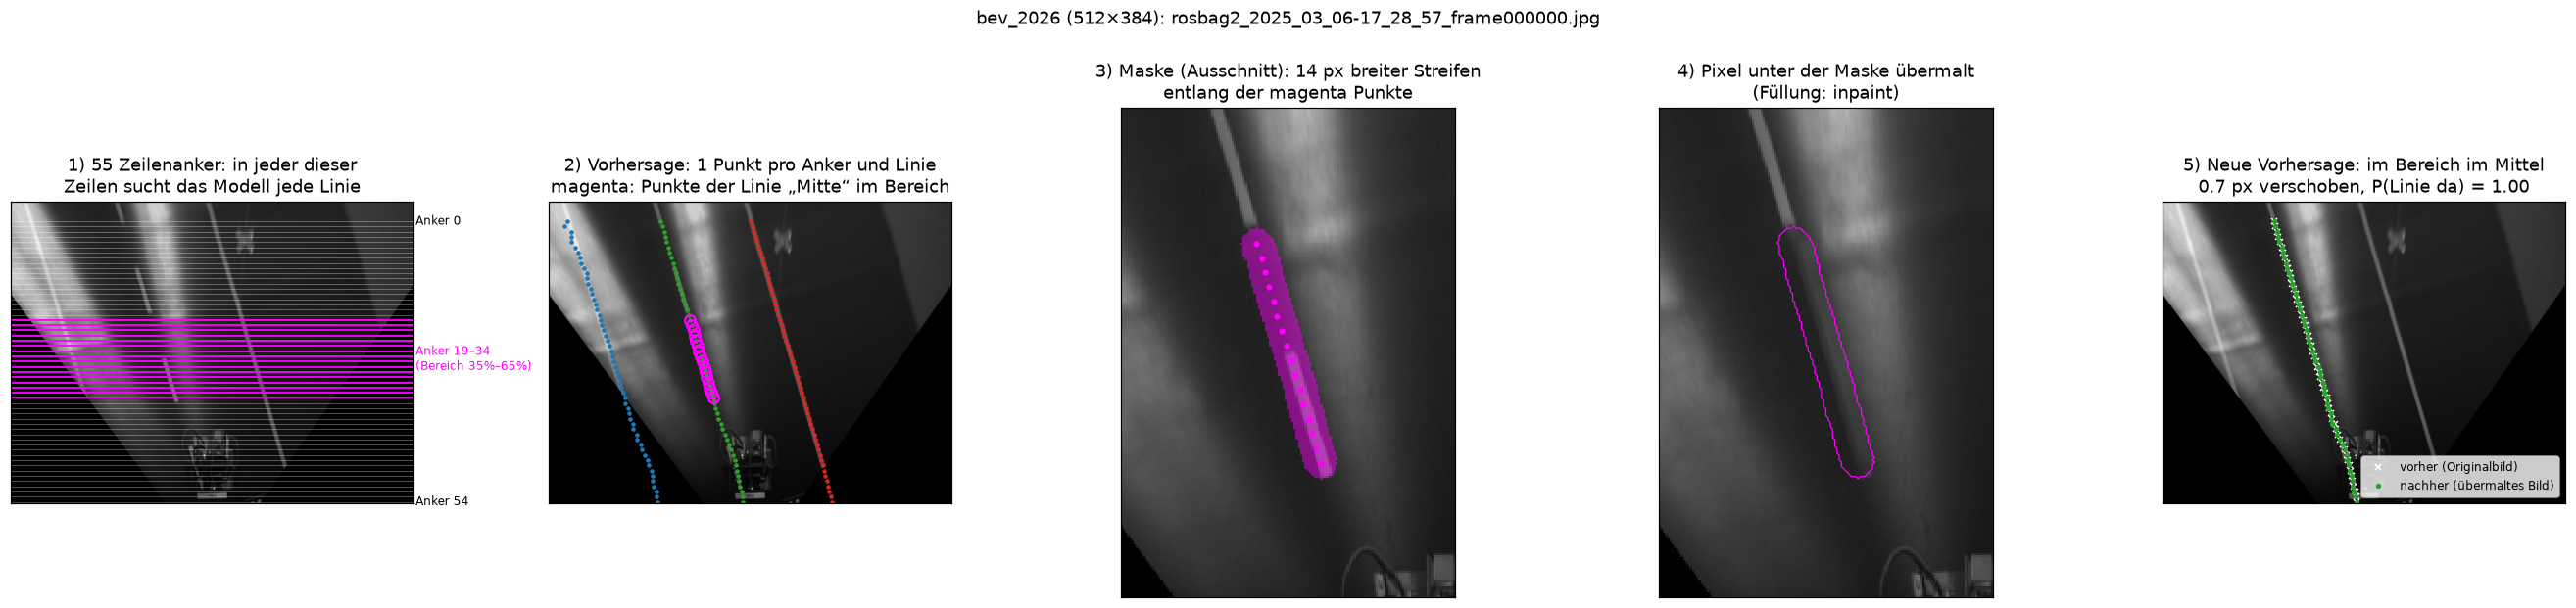
\includegraphics[width=\textwidth]{schritte_2026_inpaint.png}
\caption{Das Experiment in fünf Schritten (2026er-Modell, Bild 0, Ziellinie Mitte).}
\label{fig:schritte}
\end{figure}

\begin{enumerate}[label=\textbf{\arabic*)}]
  \item \textbf{Bereich wählen.} Wir wählen die Zeilenanker zwischen 35\,\% und 65\,\% der
        Ankerliste aus (magenta). Beim 2026er-Modell sind das die Anker 19--34, beim alten
        die Anker 12--21. Weil die Anker fast das ganze Bild abdecken, entspricht das ungefähr
        dem mittleren Drittel des Bildes.
  \item \textbf{Punkte nehmen.} Das Modell sagt auf dem \emph{Originalbild} voraus, wo die Linien
        liegen. Die Punkte der Ziellinie im gewählten Bereich (magenta Kreise) sind das Stück, das
        verschwinden soll.
  \item \textbf{Maske zeichnen.} Wir verbinden diese Punkte zu einer Linie und machen sie dick:
        14\,px bei 512\,px Bildbreite, 4\,px bei 128\,px. Diese Fläche heißt \textbf{Maske}. Sie
        liegt genau über der Markierung.
  \item \textbf{Übermalen.} Alle Pixel unter der Maske werden ersetzt (siehe unten). Danach ist
        das Stück der Linie weg.
  \item \textbf{Neu vorhersagen.} Das veränderte Bild geht noch einmal ins Modell. Wir vergleichen
        die neuen Punkte (grün) mit den alten (weiße $\times$).
\end{enumerate}

\subsection{Drei Arten zu übermalen}

\begin{description}[leftmargin=1.9cm, style=nextline]
  \item[\code{inpaint}] Die Lücke wird aus der Umgebung heraus aufgefüllt (OpenCV, Telea-Verfahren),
        wie der Reparaturpinsel in einer Bildbearbeitung. Am realistischsten und unser
        \textbf{Standard für Auswertungen}.
  \item[\code{median}] Die Fläche wird mit dem typischen Grauwert der Straße daneben gefüllt.
        Einfach, aber es entstehen flache graue Balken, die im Schatten deutlich auffallen.
  \item[\code{blendung}] Ein heller, weich auslaufender Fleck wie Sonne oder Scheinwerfer: Linie
        und Straße werden gleich hell. Das ist die Variante für die Frage nach dem
        \emph{Lichteinfall}.
\end{description}

\begin{figure}[h]
\centering
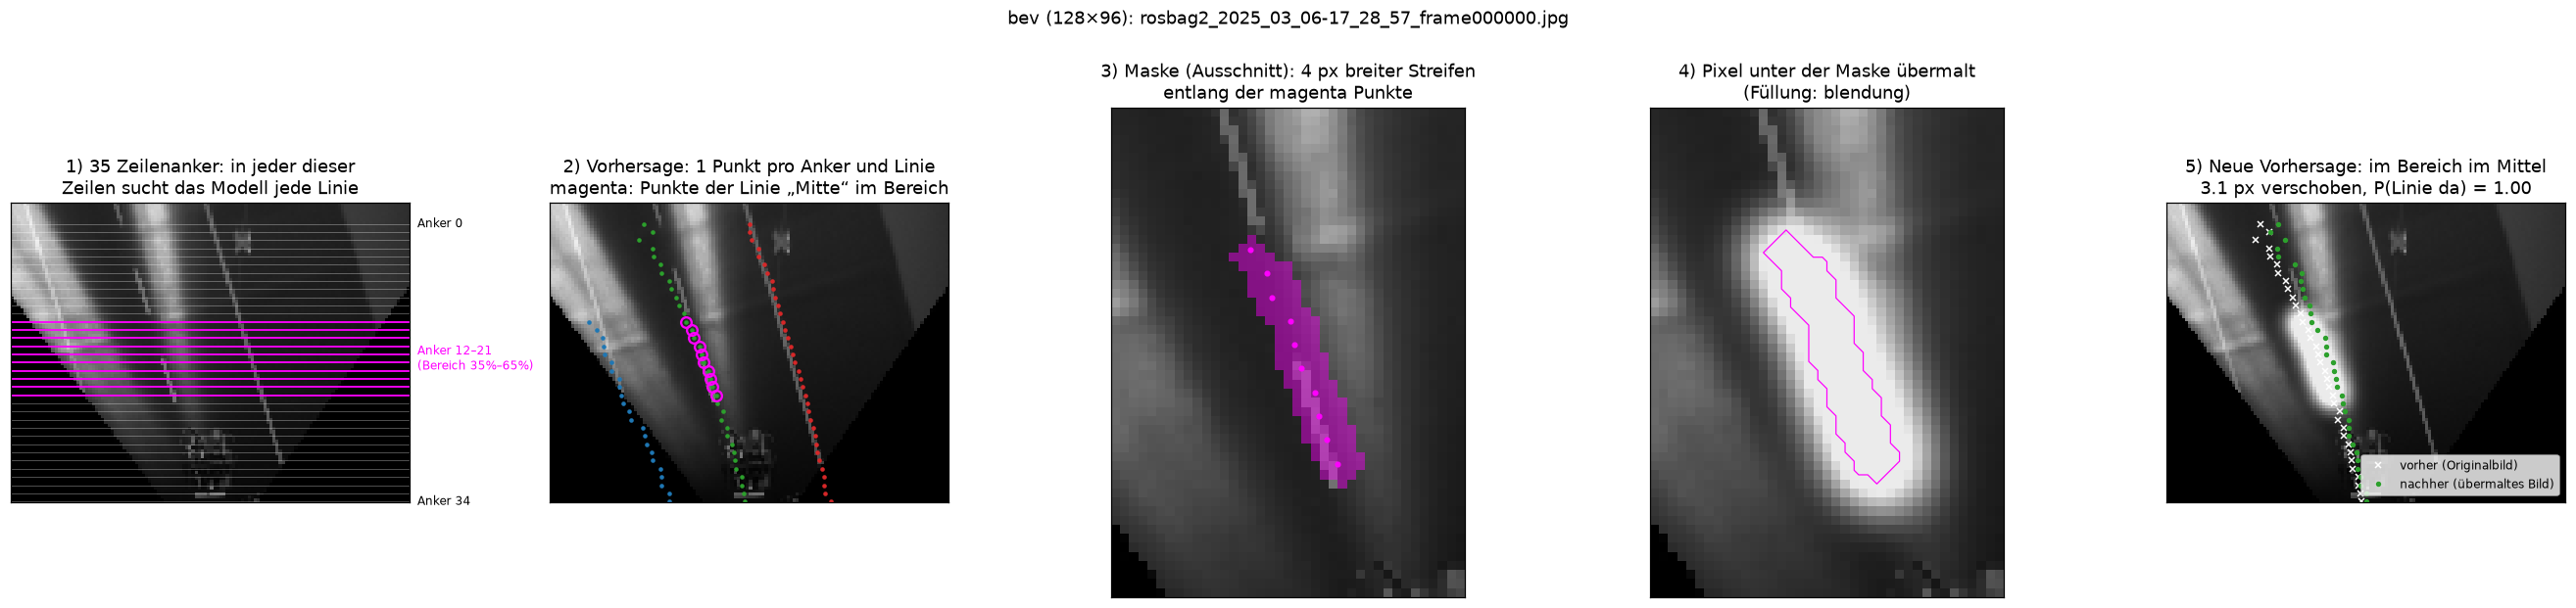
\includegraphics[width=\textwidth]{schritte_bev_blendung.png}
\caption{Dasselbe mit dem alten Modell und \code{blendung}. Man sieht, wie grob $128\times96$
Pixel sind (Schritt 3), und wie der Lichtfleck die Linie verschluckt (Schritt 4).}
\end{figure}

\begin{achtung}
Das Übermalen selbst verändert das Bild, und zwar nicht nur „Linie weg“. Ein grauer Balken oder
ein heller Fleck kann für das Modell selbst wie eine Struktur aussehen. Deshalb brauchen wir eine
\textbf{Kontrollbedingung} (D) und prüfen jede Aussage mit mindestens zwei Füllungen.
\end{achtung}

\subsection{Die fünf Bedingungen}

Für eine \textbf{Ziellinie T} und eine \textbf{Nachbarlinie N}:

\begin{center}
\begin{tabular}{clp{6.6cm}}
\toprule
& verdeckt & Frage \\
\midrule
\textbf{0} & nichts & Referenz, damit vergleichen wir alles \\
\textbf{A} & Stück von T & Wie gut schätzt das Modell die Lücke? \\
\textbf{B} & Stück von T + ganz N & Wird es schlechter, wenn auch der Nachbar fehlt? \\
\textbf{C} & nur N & Stört das Fehlen von N die \emph{voll sichtbare} Linie T? \\
\textbf{D} & Stück von T + Streifen auf freier Straße & Kontrolle: Schadet \emph{jede}
            gleich große Änderung? \\
\bottomrule
\end{tabular}
\end{center}

Der Kontrollstreifen in D hat dieselbe Form wie N, liegt aber genau in der Mitte zwischen T und
N, also auf freier Straße. D verändert damit ungefähr gleich viel Bildfläche wie B, nimmt aber
keine Linie weg.

\subsection{Wie man die Bedingungen liest}

\begin{itemize}
  \item \textbf{B deutlich schlechter als A} $\Rightarrow$ das Modell hat N genutzt.
  \item \textbf{B auch schlechter als D} $\Rightarrow$ das liegt wirklich an N und nicht daran,
        dass mehr vom Bild verändert wurde.
  \item \textbf{C schon groß} $\Rightarrow$ das Modell hängt \emph{immer} an N, auch wenn T selbst
        sichtbar ist. Das spricht für eine \textbf{gelernte Spurbreite} und nicht für ein
        gezieltes „Lücke mit Hilfe des Nachbarn füllen“.
\end{itemize}

Die letzte Unterscheidung ist feiner, als sie aussieht. Wenn B ungefähr A + C ist, addieren
sich zwei unabhängige Effekte: „T hat eine Lücke“ und „N fehlt“. Wäre B deutlich \emph{größer}
als A + C, dann bräuchte das Modell N gerade \emph{wegen} der Lücke, und das wäre die
eigentliche Antwort auf die Forschungsfrage. Formal ist das der \textbf{Interaktionseffekt}
$(B - A) - (C - 0)$.

\subsection{Was gemessen wird}

Gemessen wird nur an den Ankern des verdeckten Stücks von T:

\begin{description}[leftmargin=2.9cm, style=nextline]
  \item[\code{dx\_mittel\_px}] mittlerer Abstand der neuen x-Position zur Referenz in Pixeln der
        Modellauflösung
  \item[\code{dx\_mittel\_pct}] dasselbe in \textbf{\% der Bildbreite}. Nur damit lassen sich
        beide Modelle vergleichen, denn 1\,px bei 128\,px Breite entspricht 4\,px bei 512\,px.
  \item[\code{P\_exist\_T}] Wahrscheinlichkeit für „Linie da“, gemittelt über die Anker
  \item[\code{Anker\_verloren}] Anker, an denen das Modell die Linie gar nicht mehr findet
\end{description}

\begin{achtung}
\textbf{Die Referenz ist die Vorhersage auf dem Originalbild, nicht die Wahrheit.} Labels gibt
es keine. Wir messen also, wie stark sich das Modell durch die Verdeckung \emph{ändert}, nicht,
ob es richtig liegt. Liegt das Modell schon im Original daneben, messen wir die Änderung einer
falschen Vorhersage.
\end{achtung}

% =====================================================================
\section{Grad-CAM und HiResCAM}
\label{sec:cam}

\subsection{Die Grundidee: Class Activation Maps}

Die letzte Faltungsschicht (bei uns \code{layer4} oder \code{layer3}) hat für jede Bildzelle
$(i,j)$ und jeden Kanal $k$ einen Wert $A^k_{ij}$, die \emph{Aktivierung}. Grob gesagt: Wie stark
„sieht“ Kanal $k$ an dieser Stelle sein Muster, etwa eine helle senkrechte Kante?

Eine \emph{Class Activation Map} (CAM) kombiniert diese Kanäle zu \emph{einer} Karte: Kanäle, die
für die erklärte Ausgabe $y$ wichtig sind, bekommen viel Gewicht. Wie „wichtig“ bestimmt wird,
unterscheidet die Verfahren. Beide nutzen dazu den \textbf{Gradienten} $\partial y / \partial
A^k_{ij}$: Wie stark ändert sich $y$, wenn sich die Aktivierung an dieser Stelle ein wenig ändert?

\subsection{Was wir erklären: die Zielgröße $y$}

Eine CAM erklärt immer \emph{eine} Zahl. Bei der Bildklassifikation ist das die Punktzahl einer
Klasse („Hund“). Bei uns gibt es Tausende Ausgaben, also müssen wir wählen. Wir nehmen
\begin{equation*}
  y \;=\; \sum_{k \in \text{verdeckt}} z_{\,b^\ast_k,\,k,\,T}
\end{equation*}
also die Summe der Punktzahlen $z$, die das Modell \emph{im Originalbild} den Gewinner-Kästchen
$b^\ast_k$ der verdeckten Anker $k$ von Linie $T$ gegeben hat. Im Code heißt das
\code{RowBinTarget}.

Übersetzt fragt die Heatmap: \textbf{„Welche Bildbereiche halten das Stück von T an seiner
ursprünglichen Stelle?“} Das passt genau zum Experiment, das misst, ob das Stück nach der
Verdeckung woanders landet.

\subsection{Grad-CAM}

Grad-CAM \cite{gradcam} gibt jedem Kanal \emph{ein} Gewicht, nämlich den über alle Bildstellen
gemittelten Gradienten:
\begin{equation*}
  \alpha_k = \frac{1}{Z}\sum_{i,j} \frac{\partial y}{\partial A^k_{ij}}, \qquad
  L^{\text{Grad-CAM}}_{ij} = \mathrm{ReLU}\Big(\sum_k \alpha_k\, A^k_{ij}\Big).
\end{equation*}
Dabei ist $Z$ die Anzahl der Zellen. Die ReLU wirft negative Werte weg, denn gezeigt werden soll
nur, was $y$ \emph{erhöht}.

\subsection{HiResCAM}

HiResCAM \cite{hirescam} mittelt nicht, sondern multipliziert Gradient und Aktivierung
\textbf{Zelle für Zelle}:
\begin{equation*}
  L^{\text{HiResCAM}}_{ij} = \mathrm{ReLU}\Big(\sum_k \frac{\partial y}{\partial A^k_{ij}}\, A^k_{ij}\Big).
\end{equation*}

\subsection{Warum der Unterschied bei UFLD wichtig ist}

Bei klassischen Klassifikationsnetzen folgt auf die letzte Faltung ein \emph{Global Average
Pooling}: Alle Zellen werden gemittelt, danach kommt eine lineare Schicht. Dort ist der Gradient
für alle Zellen eines Kanals gleich, das Mitteln in Grad-CAM verliert also nichts, und beide
Verfahren liefern dieselbe Karte.

UFLD hat aber \textbf{Flatten + FC} (Kapitel 3). Jede Zelle hat ihr \emph{eigenes} Gewicht in der
FC-Schicht. Der Gradient an der Mittellinie kann also ganz anders sein als der Gradient am
Bildrand. Grad-CAM mittelt diese Unterschiede weg: Ein Kanal, der an der Mittellinie wichtig ist,
bekommt sein Gewicht über das ganze Bild verteilt. Die Karte zeigt dann auch Stellen, an denen
der Kanal zwar aktiv ist, die aber für $y$ keine Rolle spielen.

HiResCAM behält die Unterschiede. Für ein Netz, das nach der letzten Faltung nur \emph{eine}
lineare Schicht hat, ist beweisbar, dass HiResCAM genau zeigt, welche Stellen zu $y$ beitragen
\cite{hirescam}. UFLD hat zwei FC-Schichten mit ReLU dazwischen. Die Garantie gilt dann nicht
streng, HiResCAM ist aber eine lokale, positionsgenaue Näherung und deutlich treuer als
Grad-CAM.

\begin{merke}
\textbf{Grad-CAM:} ein Gewicht pro Kanal, über das Bild gemittelt $\Rightarrow$ verwischt bei
Flatten+FC-Köpfen.\\
\textbf{HiResCAM:} Gewicht pro Kanal \emph{und} Stelle $\Rightarrow$ positionsgenau.\\
Bei UFLD erwarten wir deshalb, dass HiResCAM besser zu den Experimenten passt. Genau das prüfen wir.
\end{merke}

\subsection{Die Auflösung ist das Hauptproblem}

Die Karte hat nur so viele Zellen wie die Schicht: $6\times8$ beim alten Modell (layer3),
$12\times16$ beim 2026er (layer4). Für die Darstellung wird sie auf Bildgröße hochskaliert und
weichgezeichnet, das sieht feiner aus, als es ist. Beim alten Modell ist eine Zelle etwa 16\,px
breit, mehr als der Abstand zwischen einer Linie und der Straße daneben. Man kann damit sagen
„das Modell schaut in Richtung Mittellinie“, aber nicht „genau auf die Markierung“.

\subsection{Wie wir Heatmap und Experiment vergleichen}

\begin{description}[leftmargin=2.9cm, style=nextline]
  \item[\code{N\_Anteil}] Welcher Anteil der gesamten Heatmap-Masse liegt auf der Maske von N?
  \item[\code{N\_vs\_Flaeche}] \code{N\_Anteil} geteilt durch den Flächenanteil der Maske am
        Bild. Ein Wert über 1 heißt: Die Heatmap liegt dort häufiger, als es die Größe der Fläche
        erwarten lässt. 1 wäre „zufällig verteilt“.
  \item[Spearman $\rho$] Wir berechnen über alle Bilder, wie gut \code{N\_Anteil} mit dem
        gemessenen Effekt $B - A$ zusammenhängt. Eine treue Heatmap müsste in genau den Bildern
        mehr auf N zeigen, in denen N tatsächlich hilft.
\end{description}

% =====================================================================
\section{Kurz erklärt: die Statistik}

\subsection{Warum Median?}

Die Verschiebungen sind schief verteilt: Meist ist es wenig, manchmal sehr viel. Der Mittelwert
würde von wenigen Ausreißern bestimmt. Der Median, also der mittlere Wert, wenn man alle
sortiert, beschreibt das typische Bild besser.

\subsection{Gepaart: dasselbe Bild zweimal}

Für jedes Bild haben wir A \emph{und} B. Wir vergleichen also nicht zwei Gruppen von Bildern,
sondern \emph{dasselbe Bild unter zwei Bedingungen}. Das ist viel empfindlicher, weil
Unterschiede zwischen den Bildern (hell, dunkel, Kurve, gerade) herausfallen. Pro Bild rechnen
wir die Differenz $d = \text{dx}_B - \text{dx}_A$.

\subsection{Wilcoxon-Vorzeichen-Rang-Test}

Frage: Sind die Differenzen $d$ \emph{systematisch} positiv, oder schwanken sie nur zufällig um
null? Der Test sortiert die $|d|$ nach Größe, vergibt Ränge und vergleicht die Rangsumme der
positiven mit der der negativen Differenzen. Er setzt keine Normalverteilung voraus. Wir testen
\emph{einseitig}, denn die Hypothese hat eine Richtung: „Ohne N wird es \emph{schlechter}.“

\subsection{Was ein p-Wert bedeutet}

Der p-Wert ist die Wahrscheinlichkeit, ein mindestens so deutliches Ergebnis zu sehen,
\emph{wenn es in Wirklichkeit gar keinen Effekt gäbe}. $p = 3\cdot10^{-8}$ heißt: Ohne echten
Effekt wäre so ein Ergebnis praktisch unmöglich.

\begin{achtung}
Ein kleiner p-Wert heißt \emph{nicht}, dass der Effekt groß ist, sondern nur, dass er sehr
regelmäßig auftritt. Unsere Effekte sind oft nur 1--3\,\% der Bildbreite, aber in fast jedem Bild
gleich gerichtet. Außerdem stammen alle Bilder aus \emph{einer} Fahrt, und benachbarte Bilder
ähneln sich. Die Bilder sind also nicht wirklich unabhängig, und die p-Werte sind deshalb zu
optimistisch. Wir nehmen nur jedes 20.\ Bild, um das abzumildern.
\end{achtung}

\subsection{Spearman-Korrelation}

Misst, ob zwei Größen \emph{gemeinsam steigen}, ohne dass der Zusammenhang linear sein muss. Beide
Größen werden in Ränge umgerechnet und dann korreliert. $\rho = +1$: perfekt gleichläufig;
$0$: kein Zusammenhang; $-1$: gegenläufig. Werte unter etwa $0{,}3$ gelten als schwach.

% =====================================================================
\section{Die Übersichtsabbildung lesen}

\begin{figure}[h]
\centering
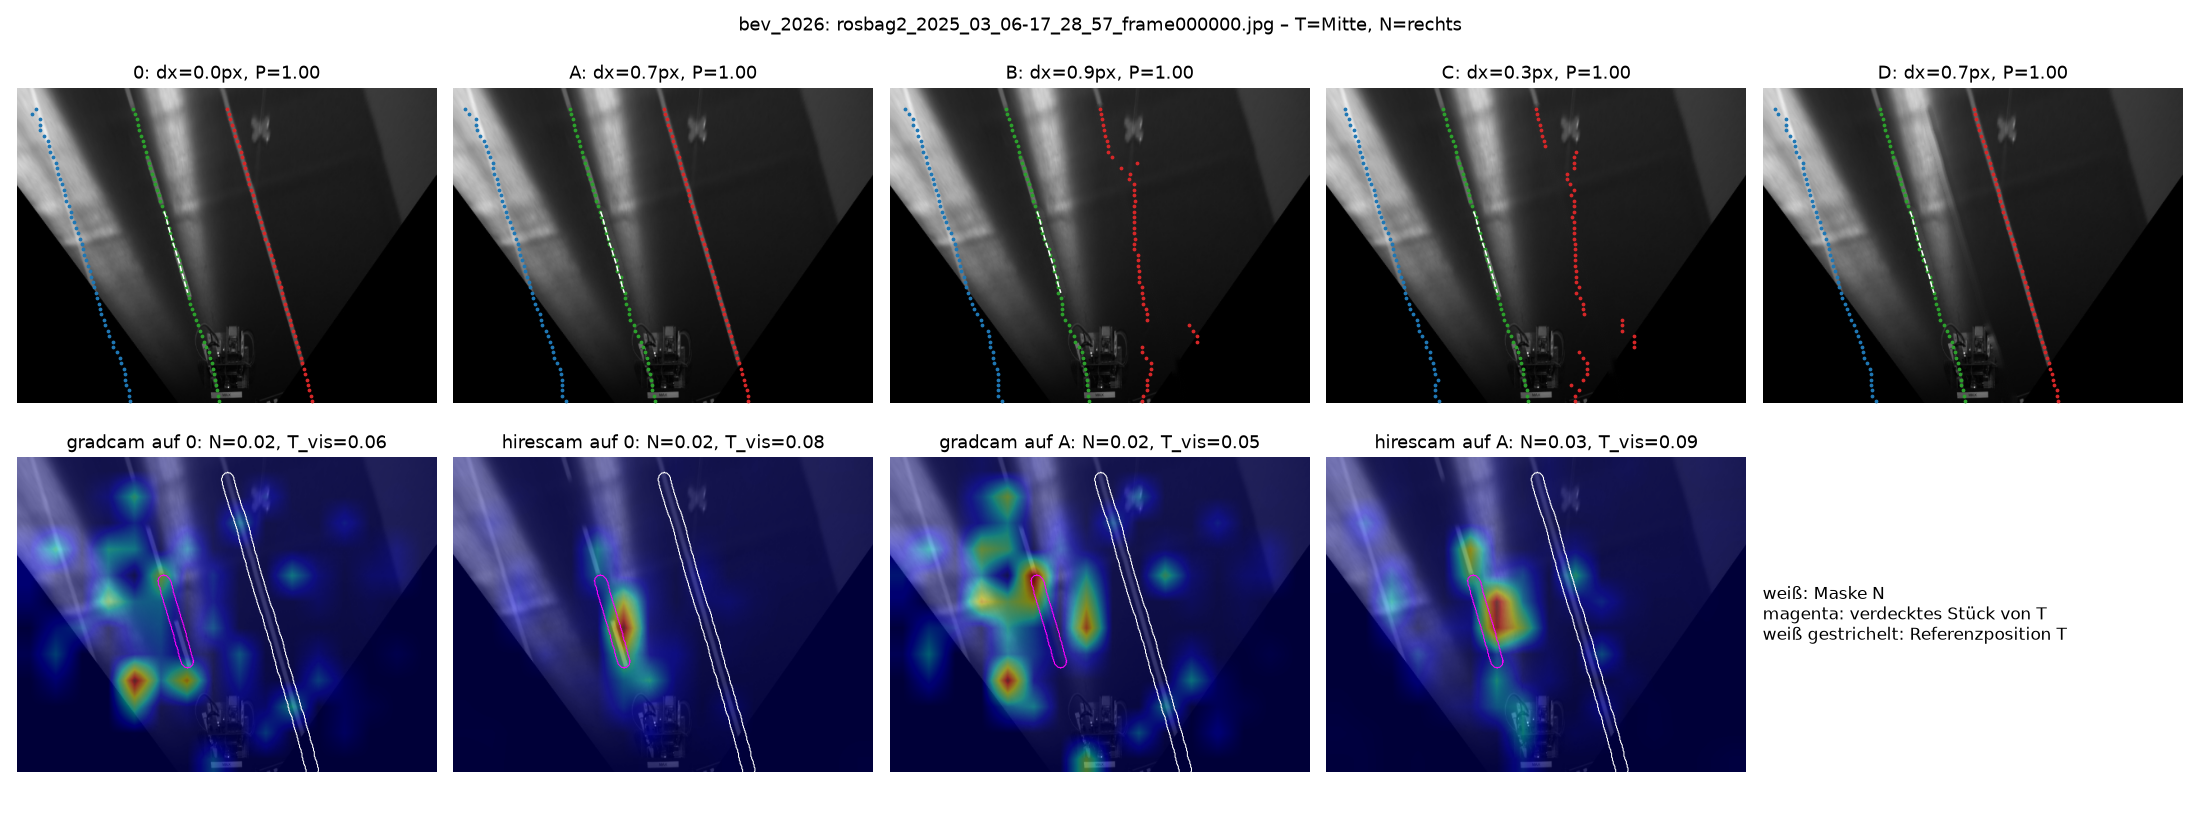
\includegraphics[width=\textwidth]{bedingungen_2026_frame0.png}
\caption{Ausgabe von \code{01\_first\_look.py}: 2026er-Modell, Bild 0, Ziellinie Mitte,
Nachbar rechts, Füllung \code{inpaint}.}
\label{fig:uebersicht}
\end{figure}

\textbf{Obere Reihe:} die fünf Bedingungen. Punkte: blau links, grün Mitte, rot rechts. Weiß
gestrichelt ist die Referenzposition des verdeckten Stücks. Im Titel stehen Verschiebung und
Sicherheit.

\textbf{Untere Reihe:} die Heatmaps für das verdeckte Stück von T, auf dem Originalbild (0) und
auf Bild A. Rot heißt wichtig. Weiß umrandet ist die Nachbarlinie, magenta das verdeckte Stück.
\code{N=0.02} heißt: 2\,\% der Karte liegen auf der Nachbarlinie.

\textbf{Was man hier sieht:}
\begin{itemize}
  \item Die Mittellinie wird auch ohne die rechte Linie fast unverändert gefunden (B kaum
        schlechter als A). Das 2026er-Modell braucht den Nachbarn hier nicht.
  \item \textbf{HiResCAM} konzentriert sich auf die Mittellinie selbst, Grad-CAM verteilt sich über
        das halbe Bild. Das ist genau der in Kapitel~\ref{sec:cam} beschriebene Effekt.
  \item Interessant: HiResCAM zeigt auf Bild A auf die \emph{übermalte} Stelle. Entweder nutzt das
        Modell dort noch Reste, oder die Karte ist zu grob, um die Lücke vom Rest der Linie zu
        trennen. Das ist offen.
\end{itemize}

% =====================================================================
\section{Ergebnisse}

\subsection{Altes Modell \code{bev}: 60 Bilder}

\begin{figure}[h]
\centering
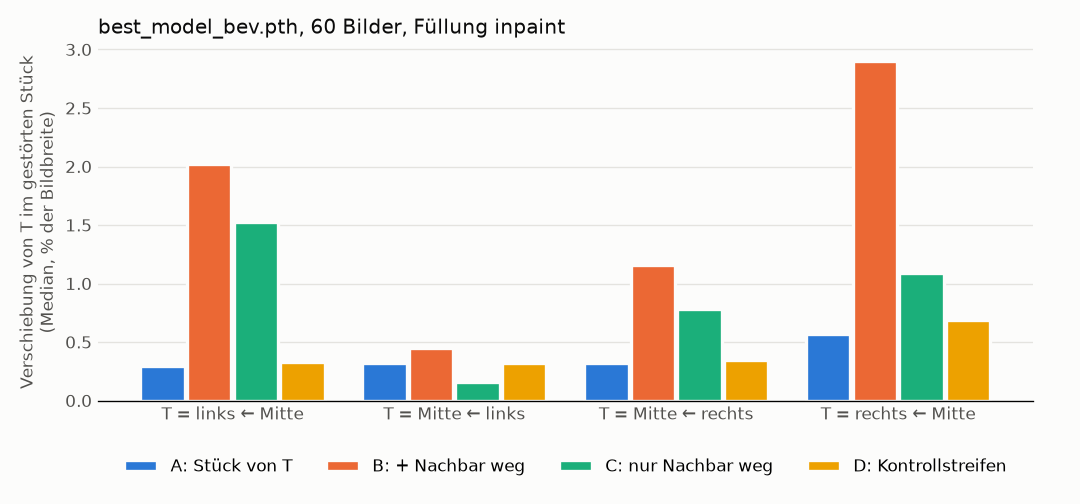
\includegraphics[width=0.92\textwidth]{batch_bev_inpaint.png}
\caption{Verschiebung des verdeckten Stücks von T (Median über die Bilder, \% der
Bildbreite), Füllung \code{inpaint}. „T $\leftarrow$ N“: Ziellinie T mit Nachbar N.}
\end{figure}

\begin{center}
\small
\begin{tabular}{lrrrrrrr}
\toprule
T $\leftarrow$ N & Bilder & A & B & C & D & $p$ ($B{>}A$) & $p$ ($B{>}D$) \\
\midrule
links $\leftarrow$ Mitte  & 50 & 0,29 & \textbf{2,02} & 1,52 & 0,33 & $3\cdot10^{-8}$  & $1\cdot10^{-6}$ \\
Mitte $\leftarrow$ links  & 56 & 0,32 & 0,45 & 0,16 & 0,32 & $2\cdot10^{-4}$  & $0{,}009$ \\
Mitte $\leftarrow$ rechts & 58 & 0,32 & \textbf{1,16} & 0,78 & 0,35 & $3\cdot10^{-10}$ & $1\cdot10^{-8}$ \\
rechts $\leftarrow$ Mitte & 59 & 0,57 & \textbf{2,91} & 1,09 & 0,69 & $8\cdot10^{-11}$ & $1\cdot10^{-9}$ \\
\bottomrule
\end{tabular}
\end{center}

\textbf{1. Das alte Modell nutzt die Nachbarlinien.} In allen vier Fällen ist B signifikant
schlechter als A \emph{und} als die Kontrolle D. Füll-Artefakte erklären das also nicht. Am
stärksten hängen die \textbf{Außenlinien an der Mittellinie}. Die Mitte hängt mehr an der
rechten als an der linken Linie, denn links fehlt oft eine echte Markierung.

\textbf{2. Es ist vor allem ein allgemeiner Effekt.} Schon C, bei dem T ganz sichtbar bleibt,
verschiebt T deutlich. Bei „links $\leftarrow$ Mitte“ ist B (2,02) etwa A + C (0,29 + 1,52 =
1,81). Die Effekte addieren sich also. Das Modell scheint eine \textbf{Spurbreite gelernt} zu
haben und setzt die Linien relativ zueinander. Dass es N \emph{speziell zum Füllen der Lücke}
nutzt, lässt sich daraus nicht ablesen.

\textbf{3. Die Effekte sind klein, aber regelmäßig.} 1--3\,\% der Bildbreite sind bei 128\,px
nur 1--4\,px. In 88--95\,\% der Bilder geht der Effekt aber in dieselbe Richtung.

\textbf{4. Die Heatmaps passen nur teilweise.}
\begin{itemize}
  \item Bei „links $\leftarrow$ Mitte“ zeigt nur \textbf{HiResCAM} überdurchschnittlich auf die
        Mittellinie, das 1,6-Fache des Flächenanteils. Grad-CAM zeigt fast nichts, das
        0,09-Fache. Hier stimmt nur HiResCAM mit dem Experiment überein.
  \item Bei „Mitte $\leftarrow$ links“ ist der Effekt klein, und beide Heatmaps zeigen fast nichts
        auf N. Das ist stimmig.
  \item Bei „rechts $\leftarrow$ Mitte“ ist der Effekt am größten, aber beide Heatmaps liegen nur
        etwa beim Flächenanteil. Hier passen die Erklärungen nicht.
  \item Pro Bild hängen Heatmap-Anteil und Effekt nur schwach zusammen ($\rho$ zwischen $-0{,}25$
        und $+0{,}45$). Die Heatmaps sagen nicht verlässlich voraus, \emph{in welchem Bild} der
        Nachbar wichtig ist. Bei $6\times8$ Zellen ist das aber auch kaum zu erwarten.
\end{itemize}

\subsection{2026er-Modell \code{bev\_2026}}
Der Batch-Lauf mit dem 2026er-Modell war bei Erstellung dieses Skripts noch nicht fertig. Die
Einzelbilder deuten darauf hin, dass es bei gut sichtbaren Linien weniger am Nachbarn hängt
(Abb.~\ref{fig:uebersicht}), bei fehlenden Linien aber stark, und dann eher die Position
verschiebt als unsicher zu werden.


\subsection{Erste Beobachtung zur Blendung}

Auf einem einzelnen Bild, also noch ohne Statistik: Liegt ein Lichtfleck auf der freien Straße
\emph{zwischen} zwei Linien (Bedingung D mit \code{blendung}), verschiebt das alte Modell die
Linie um fast \textbf{20\,\% der Bildbreite}. Das Modell hält den hellen Fleck offenbar selbst
für eine Linie. Für das Fahrzeug ist das wahrscheinlich gefährlicher als eine verdeckte Linie,
denn das Modell ist sich dabei weiter sicher.

% =====================================================================
\section{Grenzen und Denkfehler}

\subsection{Wir verdecken, wo das Modell eine Linie vermutet}

Ohne Labels folgen die Masken den \emph{Vorhersagen}. Bei gut sichtbaren Linien ist das egal,
aber nicht überall:

\begin{figure}[h]
\centering
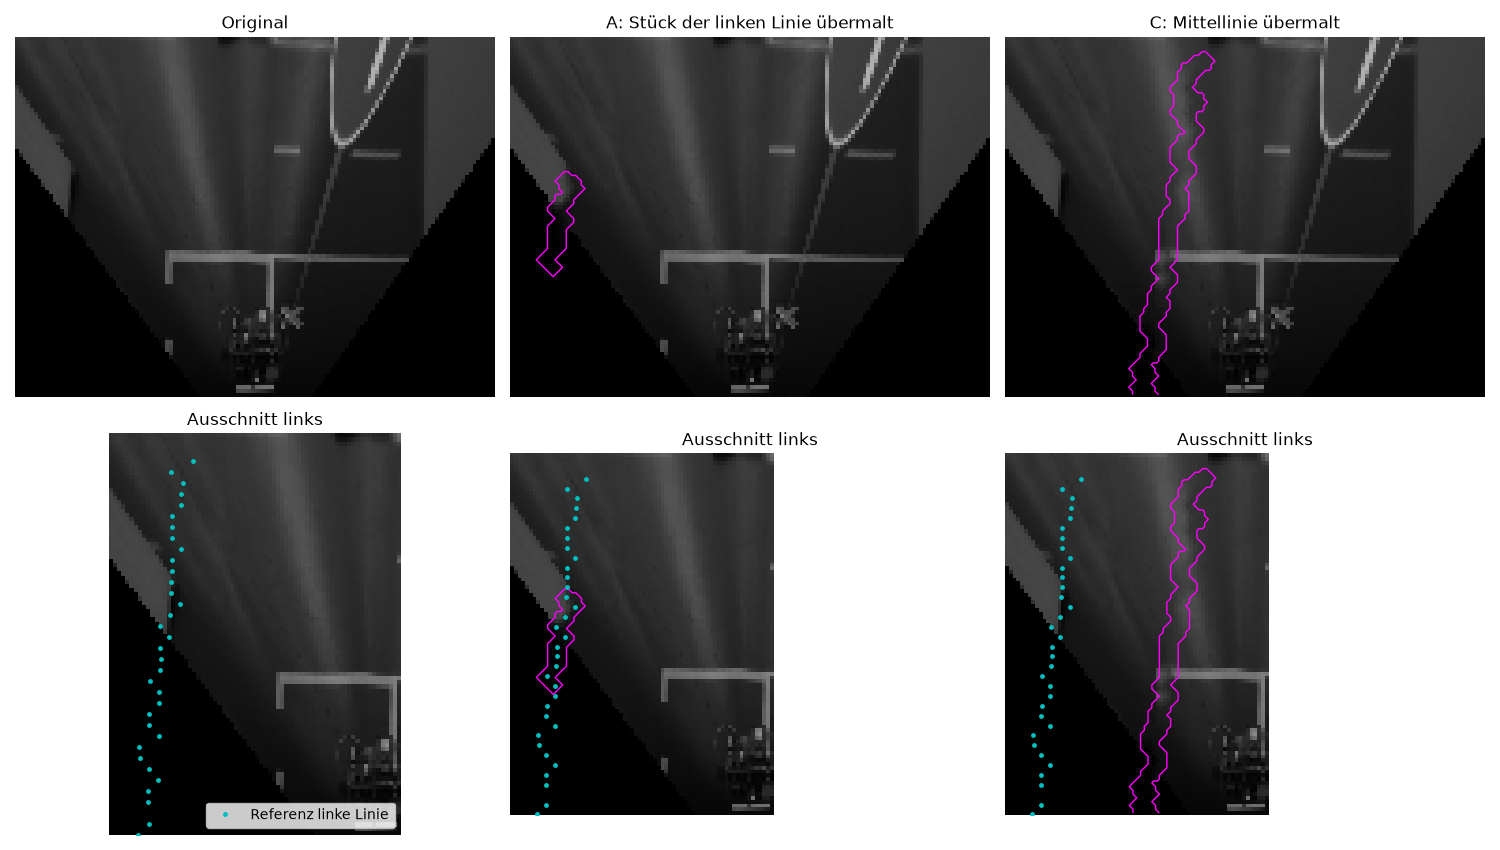
\includegraphics[width=0.95\textwidth]{masken_frame600.png}
\caption{Bild 600, altes Modell: was tatsächlich übermalt wird. Oben das ganze Bild, unten der
linke Ausschnitt. Türkis die „linke Linie“ des Modells.}
\end{figure}

\begin{itemize}
  \item \textbf{Links ist keine Markierung.} Die „linke Linie“ des Modells läuft oben an einer
        Bordsteinkante und unten am schwarzen Rand des Bildausschnitts entlang. Die Maske in A
        übermalt also nichts Relevantes, und dass dort kaum etwas passiert, ist kein Befund.
  \item \textbf{Das Bild zeigt eine Kreuzung.} Die Maske der „Mittellinie“ (C) liegt auf Straße
        und schneidet das linke Ende der Haltelinie ab. Dass die Sicherheit für links dann von
        0,86 auf 0,59 fällt, liegt vermutlich an der fehlenden Haltelinien-Ecke und nicht an einer
        fehlenden Mittellinie.
\end{itemize}

Dieses Bild zeigt also etwas anderes als die Forschungsfrage: An Kreuzungen orientiert sich das
Modell an markanten Strukturen wie der Haltelinie, und als „linke Linie“ nimmt es notfalls eine
Kante. Auch das ist ein XAI-Befund, gehört aber getrennt ausgewertet.

\subsection{Weitere Grenzen}

\begin{itemize}
  \item \textbf{Keine Labels:} Wir messen Änderung, nicht Fehler (Kapitel~\ref{sec:experiment}).
  \item \textbf{Eine Fahrt:} Alle 1192 Testbilder stammen aus einer Aufnahme vom 6.\,3.\,2025.
        Andere Strecken oder Licht können anders aussehen, und die Bilder sind nicht unabhängig.
  \item \textbf{Füll-Artefakte:} Jede Verdeckung erzeugt etwas Neues im Bild. D und mehrere
        Füllungen mildern das ab, schließen es aber nicht ganz aus.
  \item \textbf{Grobe Heatmaps:} $6\times8$ bzw.\ $12\times16$ Zellen für Linien, die nur wenige
        Pixel breit sind.
  \item \textbf{Nur Zeilenanker:} Spaltenanker werten wir nicht aus. In den Draufsichtbildern
        spielen sie kaum eine Rolle.
  \item \textbf{Ankerformel:} Ob \code{row\_anchor = linspace(100, 1540, num\_row)/1550} wirklich
        die Formel aus dem Training ist, muss das Team bestätigen. Davon hängt die Zuordnung
        Anker $\leftrightarrow$ Bildzeile ab.
\end{itemize}

\subsection{Typische Denkfehler}

\begin{achtung}
\begin{itemize}[leftmargin=1.2em]
  \item \emph{„Die Heatmap ist rot an der Mittellinie, also nutzt das Modell die Mittellinie.“}
        Nein, die Heatmap zeigt Gradienten. Ob das Modell die Stelle \emph{braucht}, zeigt erst
        das Experiment.
  \item \emph{„p ist winzig, also ist der Effekt wichtig.“} Nein, er ist regelmäßig. Wie groß er
        ist, zeigen die Prozentwerte.
  \item \emph{„B ist größer als A, also füllt das Modell die Lücke mit dem Nachbarn.“} Erst wenn B
        auch größer als A + C ist. Sonst wirkt der Nachbar einfach immer.
  \item \emph{„In Bild X passiert nichts, also ist das Modell robust.“} Erst prüfen, ob dort
        überhaupt eine echte Linie verdeckt wurde.
\end{itemize}
\end{achtung}

% =====================================================================
\section{Wie es weitergeht}

\begin{enumerate}
  \item \textbf{Sichtbarkeitsprüfung:} pro Linie und Bild prüfen, ob die Linie unter der Maske
        deutlich heller ist als die Straße daneben. Dann die Statistik getrennt für „sichtbar“
        und „geraten“ auswerten.
  \item \textbf{Kreuzungen} mit Haltelinie und Abbiegungen markieren oder ausschließen.
  \item \textbf{Interaktion} $(B-A)-C$ als eigene Kennzahl: die direkte Antwort auf die
        Forschungsfrage.
  \item \textbf{Batch mit \code{blendung}:} Robustheit gegen Lichteinfall mit Zahlen belegen.
  \item \textbf{Ausblick fürs Fahrzeug:} Mit künstlichen Lichtflecken im Training (\emph{Data
        Augmentation}) könnte das Modell lernen, Blendung zu ignorieren. Mit unseren Skripten
        lässt sich dann vorher und nachher vergleichen, ob es wirklich robuster geworden ist.
\end{enumerate}

\subsection*{Die Skripte auf einen Blick}

\begin{center}
\small
\begin{tabular}{ll}
\toprule
Skript & Zweck \\
\midrule
\code{00\_check\_setup.py} & Lädt das Modell, prüft Ausgaben und Gradienten \\
\code{01\_first\_look.py} & Ein Bild: alle Bedingungen + Heatmaps als Abbildung \\
\code{02\_batch.py} & Viele Bilder + Statistik (\code{--resume} zum Fortsetzen) \\
\code{03\_schritte.py} & Schritt-für-Schritt-Abbildung wie in Abb.~\ref{fig:schritte} \\
\code{04\_doku\_bilder.py} & Bilder für Doku und dieses Skript neu erzeugen \\
\code{interaktiv.ipynb} & Regler: Bild, Linie, Bedingung, Füllung selbst ausprobieren \\
\bottomrule
\end{tabular}
\end{center}

Alle mit \code{.venv/bin/python experiments/<skript>} im Projektordner, Modell wählen mit
\code{--model bev} oder \code{--model bev\_2026}.

% =====================================================================
\section{Glossar}

\begin{description}[leftmargin=0pt, style=sameline, itemsep=0.3em]
  \item[Ablation / Occlusion] Teile der Eingabe entfernen oder verdecken, um ihre Wirkung zu messen.
  \item[Aktivierung $A^k_{ij}$] Wert von Kanal $k$ an Stelle $(i,j)$ einer Schicht.
  \item[BEV] Bird's Eye View, Draufsicht.
  \item[Bin / Kästchen] Abschnitt einer Ankerzeile. Das Netz klassifiziert, in welchem Bin die Linie liegt.
  \item[CAM] Class Activation Map, Heatmap aus Aktivierungen und Gewichten.
  \item[FC-Schicht] Fully Connected: Jeder Eingang ist mit jedem Ausgang verbunden.
  \item[Flatten] Ein Raster zu einem langen Vektor plattdrücken. Dabei bleibt die Position als
        „welcher Eintrag“ erhalten.
  \item[Global Average Pooling] Mittelwert über alle Stellen eines Kanals. UFLD hat das \emph{nicht}.
  \item[Gradient] Wie stark sich eine Ausgabe ändert, wenn sich ein Wert leicht ändert.
  \item[Inpainting] Bildbereich aus der Umgebung heraus auffüllen.
  \item[Interaktionseffekt] Wirkung, die nur in der \emph{Kombination} zweier Eingriffe auftritt: $(B-A)-C$.
  \item[Logit] Rohe Punktzahl vor der Softmax.
  \item[Maske] Fläche, die übermalt wird.
  \item[Median] Mittlerer Wert der sortierten Werte, robust gegen Ausreißer.
  \item[p-Wert] Wahrscheinlichkeit für ein so deutliches Ergebnis ohne echten Effekt.
  \item[Referenz (Bedingung 0)] Vorhersage auf dem unveränderten Bild.
  \item[ReLU] $\max(0, x)$: negative Werte werden zu 0.
  \item[Softmax] Wandelt Punktzahlen in Wahrscheinlichkeiten um, die sich zu 1 summieren.
  \item[Spearman $\rho$] Rangkorrelation: Steigen zwei Größen gemeinsam?
  \item[Treue (Faithfulness)] Wie gut eine Erklärung das tatsächliche Verhalten des Modells wiedergibt.
  \item[Wilcoxon-Test] Prüft, ob gepaarte Differenzen systematisch in eine Richtung gehen.
  \item[Zeilenanker] Feste Bildzeile, in der das Modell jede Linie sucht.
\end{description}

% =====================================================================
\section{Selbsttest}

Versuch die Fragen erst selbst zu beantworten, bevor du die Antwort liest.

\begin{enumerate}[label=\textbf{\arabic*.}, leftmargin=1.6em]
\item \emph{Was gibt UFLD pro Zeilenanker aus?}\\
  \small Für jede der 3 Linien eine Punktzahl pro Kästchen (wo ist die Linie?) und eine
  Ja/Nein-Ausgabe (ist sie da?).\normalsize

\item \emph{Warum kann bei UFLD die Position der rechten Linie von Pixeln an der Mittellinie
  abhängen?}\\
  \small Weil der Kopf Flatten + FC nutzt: Jede Ausgabe ist mit jeder Bildzelle verbunden.\normalsize

\item \emph{Was ist der Unterschied zwischen Bedingung B und D, und warum brauchen wir D?}\\
  \small B nimmt die Nachbarlinie weg, D verändert eine ähnlich große Fläche auf freier Straße. D
  zeigt, ob jede Bildänderung schadet. Nur wenn B schlechter ist als D, liegt es am Nachbarn.\normalsize

\item \emph{C ist groß und B $\approx$ A + C. Was folgt daraus?}\\
  \small Der Nachbar wirkt immer, unabhängig von der Lücke. Das spricht für eine gelernte
  Spurbreite, nicht für gezieltes Lückenfüllen.\normalsize

\item \emph{Warum mittelt Grad-CAM bei UFLD Information weg?}\\
  \small Es gibt jedem Kanal ein über alle Stellen gemitteltes Gewicht. Bei Flatten + FC ist der
  Gradient aber an jeder Stelle anders.\normalsize

\item \emph{Was genau erklärt unsere Heatmap?}\\
  \small Die Summe der Punktzahlen der Referenz-Kästchen an den verdeckten Ankern von T, also
  „was hält dieses Stück an seiner Stelle?“.\normalsize

\item \emph{p = $10^{-10}$, Effekt 1\,\% der Bildbreite. Großer oder kleiner Effekt?}\\
  \small Klein, aber sehr regelmäßig. Der p-Wert sagt nichts über die Größe.\normalsize

\item \emph{Warum ist Bild 600 kein gutes Beispiel für die Forschungsfrage?}\\
  \small Links gibt es keine echte Markierung, und die „Mittellinie“ liegt an einer Kreuzung. Die
  Masken übermalen Kante, Schwarz und die Haltelinien-Ecke statt echter Linien.\normalsize

\item \emph{Warum vergleichen wir die Modelle in \% der Bildbreite?}\\
  \small Weil sie verschieden große Bilder sehen: 1\,px bei 128\,px Breite entspricht 4\,px bei 512\,px.\normalsize

\item \emph{Was wäre die direkte Antwort auf die Forschungsfrage, und wie misst man sie?}\\
  \small Ob der Nachbar \emph{gerade wegen} der Lücke hilft: Interaktionseffekt $(B-A)-C$,
  getrennt für Bilder mit wirklich sichtbaren Linien.\normalsize
\end{enumerate}

% =====================================================================
\begin{thebibliography}{9}
\bibitem{ufld} Z.~Qin, P.~Zhang, X.~Li: \emph{Ultra Fast Deep Lane Detection With Hybrid Anchor
  Driven Ordinal Classification.} IEEE TPAMI, 2022. (UFLDv2)
\bibitem{gradcam} R.\,R.~Selvaraju et al.: \emph{Grad-CAM: Visual Explanations from Deep Networks
  via Gradient-Based Localization.} ICCV, 2017.
\bibitem{hirescam} R.\,L.~Draelos, L.~Carin: \emph{Use HiResCAM instead of Grad-CAM for faithful
  explanations of convolutional neural networks.} arXiv:2011.08891, 2020.
\end{thebibliography}

\end{document}
